\documentclass[a4paper, 12pt, twoside]{article}


%------------------------------------------------------------------------
%
% Author                :   arcln production
% Last modification     :   2023.1.12
%
%------------------------------------------------------------------------


%------ini
\usepackage[utf8]{inputenc}
\usepackage[T1]{fontenc}
\usepackage[french]{babel}
%\usepackage[english]{babel}


%------geometry
\usepackage[textheight=700pt, textwidth=500pt]{geometry}


%------color
\usepackage{xcolor}
\definecolor{0010A1}{HTML}{0010A1}
\definecolor{00f}{HTML}{0000ff}
\definecolor{0ff}{HTML}{00ffff}
\definecolor{656565}{HTML}{656565}

%\renewcommand{\emph}{\textcolor{0010A1}}
%\renewcommand{\em}{\color{0010A1}}

\newcommand{\Emph}{\textcolor{0010A1}}

\newcommand{\strong}[1]{\textcolor{0010A1}{\bf #1}}
\newcommand{\st}{\color{0010A1}\bf}


%------Code highlighting
%---listings
\usepackage{listings}

\definecolor{cbg}{HTML}{272822}
\definecolor{cfg}{HTML}{ececec}
\definecolor{ccomment}{HTML}{686c58}
\definecolor{ckw}{HTML}{f92672}
\definecolor{cstring}{HTML}{e6db72}
\definecolor{cstringlight}{HTML}{98980f}
\definecolor{lightwhite}{HTML}{fafafa}

\lstdefinestyle{DarkCodeStyle}{
    backgroundcolor=\color{cbg},
    commentstyle=\itshape\color{ccomment},
    keywordstyle=\color{ckw},
    numberstyle=\tiny\color{cbg},
    stringstyle=\color{cstring},
    basicstyle=\ttfamily\footnotesize\color{cfg},
    breakatwhitespace=false,
    breaklines=true,
    captionpos=b,
    keepspaces=true,
    numbers=left,
    numbersep=5pt,
    showspaces=false,
    showstringspaces=false,
    showtabs=false,
    tabsize=4,
    xleftmargin=\leftskip
}

\lstdefinestyle{LightCodeStyle}{
    backgroundcolor=\color{lightwhite},
    commentstyle=\itshape\color{ccomment},
    keywordstyle=\color{ckw},
    numberstyle=\tiny\color{cbg},
    stringstyle=\color{cstringlight},
    basicstyle=\ttfamily\footnotesize\color{cbg},
    breakatwhitespace=false,
    breaklines=true,
    captionpos=b,
    keepspaces=true,
    numbers=left,
    numbersep=10pt,
    showspaces=false,
    showstringspaces=false,
    showtabs=false,
    tabsize=4,
    frame=L,
    xleftmargin=\leftskip
}

%\lstset{style=DarkCodeStyle}
\lstset{style=LightCodeStyle}
%Usage : \begin{lstlisting}[language=Caml, xleftmargin=xpt] ... \end{lstlisting}


%---Algorithm
\usepackage[linesnumbered,ruled,vlined]{algorithm2e}
\SetKwInput{KwInput}{Input}
\SetKwInput{KwOutput}{Output}

\SetKwProg{Fn}{Function}{:}{}
\SetKw{KwPrint}{Print}

\newcommand\commfont[1]{\textit{\texttt{\textcolor{656565}{#1}}}}
\SetCommentSty{commfont}
\SetProgSty{texttt}
\SetArgSty{textnormal}
\SetFuncArgSty{textnormal}
%\SetProgArgSty{texttt}

\newenvironment{indalgo}[2][H]{
    \begin{algoBox}
        \begin{algorithm}[#1]
            \caption{#2}
}
{
        \end{algorithm}
    \end{algoBox}
}


%---tcolorbox
\usepackage[many]{tcolorbox}
\DeclareTColorBox{emphBox}{O{black}O{lightwhite}}{
    breakable,
    outer arc=0pt,
    arc=0pt,
    top=0pt,
    toprule=-.5pt,
    right=0pt,
    rightrule=-.5pt,
    bottom=0pt,
    bottomrule=-.5pt,
    colframe=#1,
    colback=#2,
    enlarge left by=10pt,
    width=\linewidth-\leftskip-10pt,
}

\DeclareTColorBox{algoBox}{O{black}O{lightwhite}}{
    breakable,
    arc=0pt,
    top=0pt,
    toprule=-.5pt,
    right=0pt,
    rightrule=-.5pt,
    bottom=0pt,
    bottomrule=-.5pt,
    left=0pt,
    leftrule=-.5pt,
    colframe=#1,
    colback=#2,
    width=\linewidth-\leftskip-10pt,
}


%-------make the table of content clickable
\usepackage{hyperref}
\hypersetup{
    colorlinks,
    citecolor=black,
    filecolor=black,
    linkcolor=black,
    urlcolor=black
}


%------pictures
\usepackage{graphicx}
%\usepackage{wrapfig}

\usepackage{tikz}
%\usetikzlibrary{babel}             %Uncomment this to use circuitikz
%\usetikzlibrary{shapes.geometric}  % To draw triangles in trees
%\usepackage{circuitikz}            %Electrical circuits drawing


%------tabular
%\usepackage{color}
%\usepackage{colortbl}
%\usepackage{multirow}


%------Mathpartir (inference rules)
\usepackage{mathpartir}


%------Physics
%---Packages
%\usepackage[version=4]{mhchem} %$\ce{NO4^2-}$

%---Commands
\newcommand{\link}[2]{\mathrm{#1} \! - \! \mathrm{#2}}
\newcommand{\pt}[1]{\cdot 10^{#1}} % Power of ten
\newcommand{\dt}[2][t]{\dfrac{\mathrm d #2}{\mathrm d #1}} % Derivative


%------math
%---Packages
%\usepackage{textcomp}
%\usepackage{amsmath}
\usepackage{amssymb}
\usepackage{mathtools} % For abs
\usepackage{stmaryrd} %for \llbracket and \rrbracket
\usepackage{mathrsfs} %for \mathscr{x} (different from \mathcal{x})

%---Commands
%-Sets
\newcommand{\N}{\mathbb{N}} %set N
\newcommand{\Z}{\mathbb{Z}} %set Z
\newcommand{\Q}{\mathbb{Q}} %set Q
\newcommand{\R}{\mathbb{R}} %set R
\newcommand{\C}{\mathbb{C}} %set C
\newcommand{\U}{\mathbb{U}} %set U
\newcommand{\seg}[2]{\left[ #1\ ;\ #2 \right]}
\newcommand{\nset}[2]{\left\llbracket #1\ ;\ #2 \right\rrbracket}

%-Exponantial / complexs
\newcommand{\e}{\mathrm{e}}
\newcommand{\cj}[1]{\overline{#1}} %overline for the conjugate.

%-Vectors
\newcommand{\vect}{\overrightarrow}
\newcommand{\veco}[3]{\displaystyle \vect{#1}\binom{#2}{#3}} %vector + coord

%-Limits
\newcommand{\lm}[2][{}]{\lim\limits_{\substack{#2 \\ #1}}} %$\lm{x \to a} f$ or $\lm[x < a]{x \to a} f$
\newcommand{\Lm}[3][{}]{\lm[#1]{#2} \left( #3 \right)} %$\Lm{x \to a}{f}$ or $\Lm[x < a]{x \to a}{f}$
\newcommand{\tendsto}[1]{\xrightarrow[#1]{}}

%-Integral
\newcommand{\dint}[4][x]{\displaystyle \int_{#2}^{#3} #4 \mathrm{d} #1} %$\dint{a}{b}{f(x)}$ or $\dint[t]{a}{b}{f(t)}$

%-left right
\newcommand{\lr}[1]{\left( #1 \right)}
\newcommand{\lrb}[1]{\left[ #1 \right]}
\newcommand{\lrbb}[1]{\left\llbracket #1 \right\rrbracket}
\newcommand{\set}[1]{\left\{ #1 \right\}}
\newcommand{\abs}[1]{\left\lvert #1 \right\rvert}
\newcommand{\ceil}[1]{\left\lceil #1 \right\rceil}
\newcommand{\floor}[1]{\left\lfloor #1 \right\rfloor}
\newcommand{\lrangle}[1]{\left\langle #1 \right\rangle}

%-Others
\newcommand{\para}{\ /\!/\ } %//
\newcommand{\ssi}{\ \Leftrightarrow \ }
\newcommand{\eqsys}[2]{\begin{cases} #1 \\ #2 \end{cases}}

\newcommand{\med}[2]{\mathrm{med} \left[ #1\ ;\ #2 \right]}  %$\med{A}{B} -> med[A ; B]$
\newcommand{\Circ}[2]{\mathscr{C}_{#1, #2}}

\renewcommand{\le}{\leqslant}
\renewcommand{\ge}{\geqslant}

\newcommand{\oboxed}[1]{\textcolor{0010A1}{\boxed{\textcolor{black}{#1}}}} %orange boxed

\newcommand{\rboxed}[1]{\begin{array}{|c} \hline #1 \\ \hline \end{array}} %boxed with right opened
\newcommand{\lboxed}[1]{\begin{array}{c|} \hline #1 \\ \hline \end{array}} %boxed with left opened

\newcommand{\orboxed}[1]{\textcolor{0010A1}{\rboxed{\textcolor{black}{#1}}}} %orange right boxed
\newcommand{\olboxed}[1]{\textcolor{0010A1}{\lboxed{\textcolor{black}{#1}}}} %orange left boxed


%------commands
%---to quote
\newcommand{\simplecit}[1]{\guillemotleft$\;$#1$\;$\guillemotright}
\newcommand{\cit}[1]{\simplecit{\textcolor{656565}{#1}}}
\newcommand{\quo}[1]{\cit{\it #1}}

%---to indent
\newcommand{\ind}[1][20pt]{\advance\leftskip + #1}
\newcommand{\deind}[1][20pt]{\advance\leftskip - #1}

%---to indent a text
\newcommand{\indented}[2][20pt]{\par \ind[#1] #2 \par \deind[#1]}
\newenvironment{indt}[2][20pt]{#2 \par \ind[#1]}{\par \deind} %Titled indented env

%---title
\newcommand{\thetitle}[2]{\begin{center}\textbf{{\LARGE \underline{\Emph{#1} :}} {\Large #2}}\end{center}}

%---Maths environments
%-Proofs
\newenvironment{proof}[1][{}]{\begin{indt}{$\square$ #1}}{$\blacksquare$ \end{indt}}

%-Maths parts (proposition, definition, ...)
\newenvironment{mathpart}[1]{\begin{indt}{\boxed{\text{\textbf{#1}}}}}{\end{indt}}
\newenvironment{mathbox}[1]{\boxed{\text{\textbf{#1}}}\begin{emphBox}}{\end{emphBox}}
\newenvironment{mathul}[1]{\begin{indt}{\underline{\textbf{#1}}}}{\end{indt}}

\newenvironment{theo}{\begin{mathpart}{Théorème}}{\end{mathpart}}
\newenvironment{Theo}{\begin{mathbox}{Théorème}}{\end{mathbox}}

\newenvironment{prop}{\begin{mathpart}{Proposition}}{\end{mathpart}}
\newenvironment{Prop}{\begin{mathbox}{Proposition}}{\end{mathbox}}
\newenvironment{props}{\begin{mathpart}{Propriétés}}{\end{mathpart}}

\newenvironment{defi}{\begin{mathpart}{Définition}}{\end{mathpart}}
\newenvironment{meth}{\begin{mathpart}{Méthode}}{\end{mathpart}}

\newenvironment{Rq}{\begin{mathul}{Remarque :}}{\end{mathul}}
\newenvironment{Rqs}{\begin{mathul}{Remarques :}}{\end{mathul}}

\newenvironment{Ex}{\begin{mathul}{Exemple :}}{\end{mathul}}
\newenvironment{Exs}{\begin{mathul}{Exemples :}}{\end{mathul}}


%------Sections
% To change section numbering :
% \renewcommand\thesection{\Roman{section}}
% \renewcommand\thesubsection{\arabic{subsection})}
% \renewcommand\thesubsubsection{\textit \alph{subsubsection})}

% To start numbering from 0
% \setcounter{section}{-1}


%------page style
\usepackage{fancyhdr}
\usepackage{lastpage}

\setlength{\headheight}{18pt}
\setlength{\footskip}{50pt}

\pagestyle{fancy}
\fancyhf{}
\fancyhead[LE, RO]{\textit{\textcolor{black}{\today}}}
\fancyhead[RE, LO]{\large{\textsl{\Emph{\texttt{Cahier Des Charges}}}}}

\fancyfoot[RO, LE]{\textit{\texttt{\textcolor{black}{Page \thepage /}\pageref{LastPage}}}}
\fancyfoot[LO, RE]{
\includegraphics[scale=0.12]{arcln}}


%------init lengths
\setlength{\parindent}{0pt} %To avoid using \noindent everywhere.
\setlength{\parskip}{3pt}

% Mise en page française
\usepackage[utf8]{inputenc}
\usepackage[french]{babel}
\usepackage{geometry}

% Import d'images, couleurs
\usepackage{graphicx,color}

\usepackage{lipsum}

\newcommand{\hsp}{\hspace{20pt}}
\newcommand{\HRule}{\rule{\linewidth}{0.5mm}}

%---------------------------------Begin Document
\begin{document}

    
\begin{titlepage}
  \begin{sffamily}
  \begin{center}

  
    
\includegraphics[scale=0.3]{logo}~\\[1.5cm]

    \textsc{\LARGE EPITA Rennes}\\[0.5cm]

    % Titre
    \textsc{\Large CAHIER DES CHARGES DU PROJET S2}\\[1.5cm]

    \HRule \\[0.4cm]
     { \huge \bfseries  A Slime's Journey \\[0.4cm] }

    \HRule \\[2cm]
    
\includegraphics[scale=0.4]{arcln}
     \\[0.5cm]
    %\textsc{\Large ARCLN}\\[1.5cm]

    % Membres
    \begin{minipage}{0.4\textwidth}
      \begin{flushleft} \large
        Alexis LE GALL\\
        Enzo JUHEL\\
      \end{flushleft}
    \end{minipage}
    \begin{minipage}{0.4\textwidth}
      \begin{flushright} \large
        Maxime DOUILLARD\\
        Omid SHEIBANIFAR\\
      \end{flushright}
    \end{minipage}

    \vfill

  \end{center}
  \end{sffamily}
\end{titlepage}


    \tableofcontents
    \newpage

    \begin{indt}{\section{Introduction}}
        Dans ce cahier des charges nous allons présenter notre projet de jeux vidéo, “A Slime's Journey” développé par la compagnie ARCLN prod. Ce projet est réalisé dans le cadre du projet du second semestre d'Epita. Il est réalisé par Enzo Alexis Le Gall, Enzo Juhel, Omid Sheibanifar et Maxime Douillard. Ce jeu est un platformer 2D reliant histoire et énigmes et se déroulant dans un univers médiéval.

        Le joueur prendra donc le contrôle d'un slime, une sorte de blob qui peut se déplacer avec des petits sauts. De plus, ce slime pourra aussi faire de plus grands sauts afin de changer de plate-forme. Afin de vaincre ses ennemis, le slime pourra, au cours de son épopée, ramasser certaines armes et s'en servir. Les armes auront une rareté, différentes statistiques et seront plus efficaces selon l'ennemi affronter.

        Au contact de certains objets ou certaines matières, notre créature pourra se transformer pour avancer dans le niveau. Certains niveaux se termineront sur un combat de boss et il faudra redoubler de vigilance pour terrasser ceux ci. Les boss auront des capacités uniques, plus de vie et infligeront plus de dégâts que les monstres habituels. Une intelligence artificielle sera implémentée pour avoir des monstres qui essayeront de tuer le joueur, afin de  compliquer sa tâche dans son aventure et proposer une difficulté réelle. Cela permet aussi un gameplay nerveux, demandant de la concentration et de la maîtrise.

        L'histoire se déroule de manière épisodique et un ou plusieurs nouveaux niveaux sortiront à chaque soutenance, cette manière de dérouler l'histoire permet d'implémenter une vraie expérience narrative sans forcément de cinématiques. D'un point de vue artistique, nous essaierons de rendre le jeu agréable à la vue et à l'ouïe, pour à la fois faire comprendre au joueur ce qu'il se passe, où il se trouve, quel est son but final, et, comprendre toute l'essence de l'histoire sans intervention scénaristique, tout en restant dans la lignée des jeux de plate-formes, c'est-à-dire rester à un certain niveau de difficulté élevé pour que le joueur aie une expérience complète. Afin d'arriver à la fin du jeu, le joueur devra terminer chaque niveau, ce qui veut dire survivre jusqu'au prochain biome.

        Ce jeu pourra être joué en coopération par le biais d'un mode multijoueur en ligne. Cela permettra de découvrir ou redécouvrir le jeu avec un autre joueur. Malgré la présence d'un second joueur, la difficulté des niveaux ne changera pas. Comme le premier joueur, le deuxième joueur pourra incarner un slime qui possédera les mêmes capacités que le premier joueur.

    \end{indt}

    %\vspace{24pt}

    \begin{figure}[h!]
        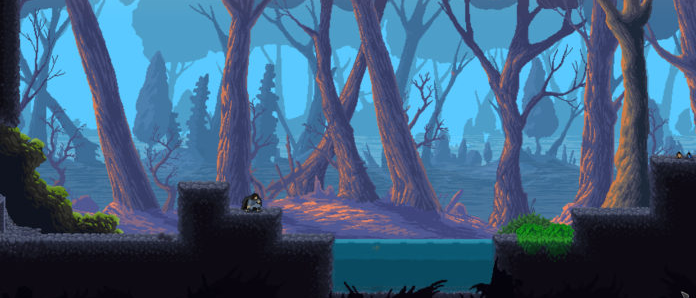
\includegraphics[width=\linewidth]{forest.png}
    \end{figure}
    
    \newpage

    \begin{indt}{\section{Plan}}
        \begin{indt}{\subsection{Origine et nature du sujet}}
            Ayant tous joué à des jeux de plateformes 2D durant notre enfance, tel que Super Mario Bros, le il s'est avéré que c'était un type de jeu que nous connaissons tous très bien et avec de nombreuses références permettant une maîtrise du sujet. De plus, une créature fantastique simple mais au caractère divers, le slime, nous a paru une évidence d'où sa place de héros dans le jeu. Sans oublier que les power up, l'exploration, les combats $\&$ Co font partie de l'univers des jeux vidéo et permettent un niveau d'immersion supérieur. D'ailleurs un autre aspect des jeu vidéos sont leur univers, mieux ceux-ci sont construit, mieux le joueur va s'y retrouver immergé, pour cela, nous avons pris la liberté de construire un univers, un histoire et une intrigue se développant tout au long des différents niveaux et qui sera assimilable par le joueurs au travers le l'aspect d'exploration du jeu. C'est ainsi que nous avons donc décidé de partir ce ce modèle de jeu vidéo, un simple plateformer 2D renfermant une histoire profonde répartie sur plusieurs niveaux.
        \end{indt}

        \begin{indt}{\subsection{Inspirations}}
            Dès l'entrée en jeu, décors et personnages seront cartoonesque, inspiré d'un autre jeu vidéo nommé Cuphead, dont imagé ci-dessous. De plus, au cours de l'aventure, des pouvoirs seront attribués au héros, le slime, ceux-ci sont issus d'un mixte des saga “Super Mario Bros” et “Kirby's Adventure”. C'est-à-dire que le héros aura la capacité de changer de forme, comme Kirby le fait en absorbant des objets spécifiques et que ses nouvelles formes offriront au joueurs de nouvelles capacités lui permettant de franchir des obstacles comme dans Mario. Enfin, tout au cours de l'aventure, une histoire se déroule à la façon de “Limbo”, l'objectif est de faire parvenir les informations au fur et à mercure et sans texte explicite au cinématique. Mais plutôt de laisser chercher au joueurs lui-même ces infos là et récompenser son exploration par des éléments participant à la compréhension de cet univers.
        \end{indt}

        \begin{center}%[h!]
            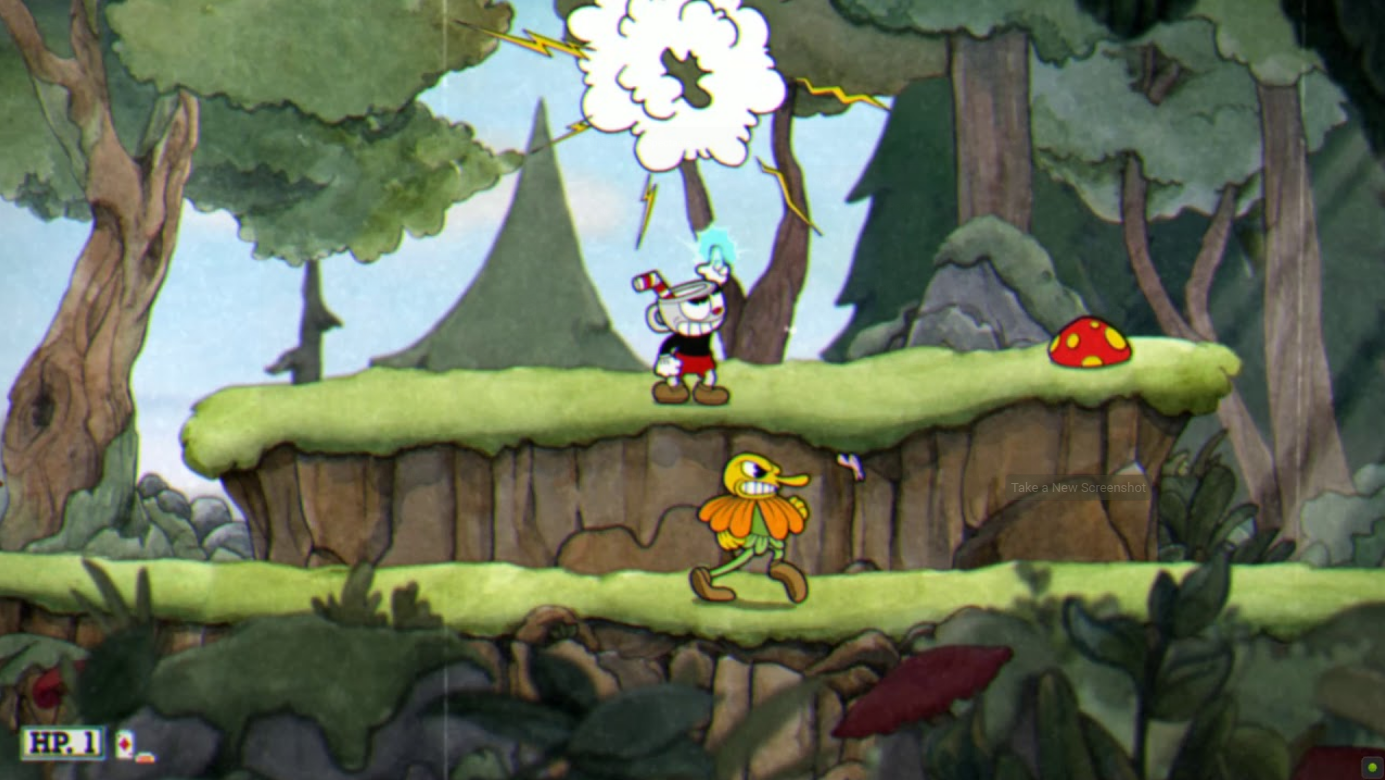
\includegraphics[width=0.8\textwidth]{Cuphead.png}
        \end{center}

        \begin{indt}{\subsection{Objet de l'étude}}
            L'un des atouts des jeux vidéo sont leur diversité d'objectifs, que se soit ceux fournit par le jeu, c'est-à-dire finir le jeu en récupérant tout ce que le jeu a à nous offrir. Mais aussi ceux créés par la communauté : compléter le jeu le plus vite possible, se priver de certains pouvoirs et bien d'autres. De plus, la difficulté du jeu sera adaptable afin que chacun puisse s'amuser. Que ce soit seul ou à deux, car jeu sera disponible en coopération afin de vivre ou revivre l'aventure avec votre meilleur acolyte. 

            D'autre part, cela constitue pour les développeurs un vrai défi créatif et enrichissant que ce soit en termes de style de niveaux, de coopération et de développement de projet. Ce projet permet à la fois de développer des compétences théoriques et pratiques. Le développement d'un jeu est à la fois un expérience de créativité, d'inventivité mais surtout d'accomplissement de projets. Il est primordial pour tout développeur de savoir délimiter et cadrer son projet de façon à le finir dans les temps tout en étant en concordance avec les attendus initiaux. Les difficultés ne relèvent pas que de l'aspect pratique mais aussi de la gestion du temps et du travail de chacun.
        \end{indt}

        %\newpage

        \begin{indt}{\subsection{Etat de l'art}}
            Le premier jeu de type plate-formes est apparu en 1980 et porte le nom de Space Panic, édité par Universal, mais ce jeu ne permettait pas au joueur de sauter. En 1981, Nintendo sort le jeu Donkey Kong sur borne arcade, qui devient le premier jeu permettant au joueur de sauter par-dessus des obstacles et de franchir des précipices, devenant ainsi le premier jeu de plates-formes à proprement parler. A partir de 1982, de nombreux jeux de plates-formes voient le jour, comme Pitfall sur Atari 2600, Manic Miner, Jet Set Willy, Impossible Mission ou encore Prince of Persia. En 1985, Super Mario Bros. nait, il se vend à plus de 40 millions d'exemplaires et devient la norme des jeux de type plates-formes. En 1990, les jeux de plates-formes font leur apparition sous la forme de jeux 3D, comme Super Mario 64 en 1996. Ce type de jeu est toujours d'actualité, en effet, de nombreux jeux sortent encore, comme Super Meat Boy en 2010, de nouveaux jeux de la série Super Mario Bros, et bien d'autres.
        \end{indt}

        \newpage
        
        \begin{indt}{\subsection{Découpage du projet}}
            Un projet d'une telle ampleur nécessite une organisation sans faille afin de pouvoir tenir ces deadlines et garder un rythme de travail constant. C'est pourquoi, le développement se partage entre 4 aspects intimement liés, la communication, le management, la programmation et le design. Le premier reflétant les échanges extérieurs des nouveautés, géré par Alexis et Maxime, que ce soit par la réalisation de trailers sur Youtube ou des annonces sur divers réseaux sociaux. Avec Enzo à la rédaction des différents documents à réaliser au cours du semestre. Ensuite, la supervision de l'équipe, réalisée à l'aide de Alexis, consiste à la prise de décisions, notamment lors de la réalisation de deadlines, répartition des tâches, etc. Puis, le code en lui-même sera rédigé par tous les membres au vu de la quantité de travail à effectuer. Enfin, la dernière section, et pas des moindres puisqu'il s'agit d'un point clé du développement, est elle aussi régie par toute l'équipe, dont chaque membre ont leurs spécialités, tel que Maxime pour la modélisation des sprites sur Gimp, ou bien Enzo capable d'élaborer des niveaux dans Unity et encore, Omid pour le choix et la composition de musiques avec Audacity. En bref, voici un planning détaillé de répartition des tâches :
            \begin{center}
                \begin{tabular}{|c|c|c|c|c|}
                    \hline
                    & Alexis & Enzo & Maxime & Omid
                    \\
                    \hline
                    Développement & Participant & Participant & Responsable & Suppléant
                    \\
                    \hline
                    Communication & Suppléant & & Responsable &
                    \\
                    \hline
                    Design & & Responsable & Suppléant &
                    \\
                    \hline
                    Audio & Suppléant & & & Responsable
                    \\
                    \hline
                    IA & Responsable & & & Suppléant
                    \\
                    \hline
                    Réseau & Responsable & Suppléant & Participant & Participant
                    \\
                    \hline
                    Rédaction & Participant & Responsable & Participant & Suppléant
                    \\
                    \hline
                \end{tabular}
            \end{center}
        
        \end{indt}

    \end{indt}

    %\vspace{12pt}

    \newpage

    \begin{indt}{\section{Présentation}}
        \begin{indt}{\subsection{Scénario}}
            Vous vous réveillez en plein milieu d'une forêt paisible, vous voici dans la peau d'un slime, un petit être rond, c'est alors qu'en commençant à comprendre comme votre nouveau corps fonctionne, que vous sortez petit à petit de cette belle forêt. Dès lors, un petit village apparaît en face et vous pouvez apercevoir au loin un immence château. En croisant les villageois, vous comprenez que tous rêvent de pouvoir pénétrer dans ce palais. C'est alors que vous vous lancez dans un grand périple rempli de danger à franchir à l'aide de votre pouvoir, celui de prendre la forme de votre environnement, vous octroyant ainsi de nouvelles capacités tel que franchir une falaise, voler et bien d'autres… De plus, le jeu permettra aux joueurs de découvrir par eux-même les secrets du royaume, en passant par ses décors et ses habitants, le tout accompagné de musique, permettant une immersion totale.
        \end{indt}
        
        \begin{indt}{\subsection{Gameplay}}
            Le jeu sera composé de deux phases, la sélection de niveau et la réalisation du niveau. Lors de la sélection du niveau, le jeu aura une vue de trois quart, nous permettant de nous déplacer dans un monde restreint et de résoudre certaines énigmes. Lors de la réalisation du niveau, le jeu sera en 2D, vue de côté, comme la majorité des jeux de plateformes.

            Les joueurs pourront acquérir temporairement différentes capacités suivant la surface sur laquelle ils se trouvent, leur permettant ainsi de surmonter certains obstacles, ou d'esquiver des ennemis. Par exemple, lorsqu'un joueur se trouve sur une montagne, son slime prendra la forme d'un pique afin de se planter dans la montagne, lui donnant ainsi la possibilité de grimper à la montagne. 

            Enfin, les joueurs pourront vaincre des monstres se trouvant sur leur passage à l'aide d'équipement ramassé au préalable durant les précédents niveaux, ou à l'aide de leurs capacités temporaires. Ce jeu est un jeu de plateformes, par conséquent, le fait de tomber dans le vide fait instantanément. Le fait de mourir, que ce soit en tombant ou en trépassant face à un monstre, le joueur perd une vie si il est en coopération et doit recommencer le niveau si il joue en solo, en coopération, si les deux joueurs meurent simultanément, le niveau devra également recommencer.

            A slime's journey comporte différents niveaux de difficultés, modifiant l'équipement obtenable, la quantité de vie des joueurs et des monstres, ainsi que les dégâts de ces derniers. Les ennemis seront gérés par des IAs différentes suivant la difficultées choisie. Il existe différents types d'items permettant de devenir plus résistants, avoir une meilleure portée d'attaque, de meilleurs dégâts, afin de vaincre de nouveaux ennemis de plus en plus coriaces. Les ennemis rencontrés au fur et à mesure de l'aventure dépendent de l'environnement du niveau, et permettent aux joueurs d'obtenir de l'équipement adapté à cet environnement.
        \end{indt}
    \end{indt}

    \newpage

    \begin{indt}{\section{Structure}}
        \begin{indt}{\subsection{Technologies et méthodologies}}
            Du point de vue de la production, l'essentiel du travail se fera sur nos pc, le jeu étant codé en C$\#$, les IDE utilisés sont Riders et Visual Studio Code, le tout fonctionnant avec Dotnet 7.0 tournant sous Windows 11 et Fedora 37. Pour ce qui est de la rédaction des différents documents nécessitant un rendu, ils seront tous rédigés en LaTeX via OverLeaf et Visual Studio Code. Par ailleurs, le moteur de jeu Unity, Github et Discord amélioreront la qualité du travail au sain du développement. D'autres logiciels notables sont Gimp, Audacity pour leur rôles respectif d'édition d'image et de musique. Le jeu étant constitué d'une série de niveaux, sera réalisable en solitaire ou en coopération avec un acolyte en utilisant un clavier et une souris ou une manette de console. Une fois le jeu lancé, le level design sera réalisé grâce à Unity, les sprites cartoon fabriqué dans Gimp, et sons d'ambiance avec Audacity permettent une immersion directe, qui plus est qu'un minimum d'action seront réalisable par le joueur, tel que se déplacer, sauter et se transformer. L'exploration de niveaux sera régi par son sens conventionnel, qui est que l'objectif se trouve toujours vers la droite mais celui-ci sera challengé par les différents monstres présents dans le niveaux, tous possédants une IA leurs permettant de contrer le joueurs dans sa progression grâce à un système de vie, faisant que dès qu'une attaque ennemi atteint le héro ou que celui-ci tombe des plateformes, il perd une vie et dois recommencer le niveau en cours. Une fois arrivé à la fin de certains niveaux, un boss fonctionnant avec une IA plus développée que les montres traditionnels, bloquera l'accès à la suite de l'aventure.
        \end{indt}

        \begin{indt}{\subsection{Fonctionnel}}
            La réalisation du projet jeu vidéo, se fera par une sortie à chaque soutenance d'au moins un nouveau niveau dont le premier mettra en avant un tutoriel et une partie exploration. L'objectif est que la difficulté à chaque nouvelle sortie soit en adéquation avec l'expérience du joueur au sain du jeu, c'est pour cela que les premiers niveau sont plus orienté vers l'exploration, la découverte et la compréhension de l'univers dans lequel le héros se trouve, tandis qu'en s'approchant de la fin, se seront plutôt l'agilité et le combat qui seront de mise. Un autre aspect qui sera développé tout au long des différents rendus sont les pouvoirs du héros, comme dit précédemment, le slime peut changer de forme selon l'environnement dans lequel il se trouve, lui donnant donc de nouvelles capacités offrant ainsi une diversité d'actions. Ainsi, l'implémentation des notions de vie et de boss de fin de certain niveaux permettent d'évaluer les capacités du joueur, car ceux ayant pris du temps de garder la forme du slime la plus adéquate à la fin et n'ayant pas perdu de vies seront avantagés pour compléter le niveau en question. Sans oublier que la coopération avec le joueur rejoignant la partie aide grandement l'avancée de la partie. Pour ce qui est du contenu en dehors du jeu lui-même, en plus du détail complet des nouveautés disponibles sur le site web officiel, chaque niveau aura le droit à un post sur Internet, que ce soit par un trailer Youtube, une annonce sur le Discord ou Instagram de l'équipe.
        \end{indt} 

        \begin{indt}{\subsection{Opérationnel}}
            Cependant un tel jeu à des coûts monétaires, car chaque membre du groupe paye un logement sur Rennes, c'est pourquoi il faut comptabiliser le coût de repas quotidiens, loyer, factures d'électricité, d'eau, etc. A part ça, une grosse partie du travail se fera sur le campus d'Epita et l'ensemble des logiciels utilisés sont gratuit ou utilisent des licences comprisent par l'école, limitant ainsi les frais.
        \end{indt} 
    \end{indt}

    %\newpage

    \begin{indt}{\section{Avancement du projet}}
        L'objectif fixé pour la première soutenance est de mettre au point au moins une IA servant aux différents ennemis. Avec cela un premier niveau sera disponible, servant à la fois de didacticiel et permettant de découvrir la base de l'histoire du jeu. Ainsi, un certain nombre de sprites, décors et musiques seront réalisés en concordance avec le style cartoon du jeu. De plus, il sera possible de réaliser les niveaux avec 2 joueurs en coopération. Du côté communication, un site web présentant le projet créé et fonctionnel.

        Ensuite, un 2nd niveau prolongera l'histoire du jeu, faisant suite au didacticiel avec l'ajout d'un boss à la fin. Côté site web, celui-ci sera mis à jour et des comptes sur les réseaux sociaux seront créés afin de publier les avancées du jeu, le tout réalisé avant la seconde soutenance.

        Enfin, à la dernière soutenance sera réalisé un site web complet permettant de télécharger le jeu pour y jouer sous Windows. Le jeu à ce moment-là sera fini, avec de nouveaux niveaux et l'ajout de fonctionnalités de gameplay tel que un mode versus.

        \begin{center}
            \begin{tabular}{|c|l|l|l|}
                \hline
                & Première Soutenance & Deuxième soutenance & Troisième soutenance
                \\
                \hline
                Développement 
                & \begin{tabular}{l}
                    $\bullet$ 1 niveau 
                    \\ 
                    $\bullet$ Interactions basiques 
                    \\ 
                    $\bullet$ 1 transformation
                \end{tabular}
                & \begin{tabular}{l}
                    $\bullet$ Second niveau
                    \\ 
                    $\bullet$ Nouvelles formes
                    \\ 
                    $\bullet$ 1 boss
                \end{tabular}
                & \begin{tabular}{l}
                    $\bullet$ Ajout derniers niveaux
                    \\ 
                    $\bullet$ Mode boss rush
                \end{tabular}
                \\
                \hline
                Communication 
                & \begin{tabular}{l}
                    $\bullet$ Site Web
                \end{tabular}
                & \begin{tabular}{l}
                    $\bullet$ Réseaux sociaux
                \end{tabular}
                & \begin{tabular}{l}
                    $\bullet$ Sortie officielle du jeu
                \end{tabular}
                \\
                \hline
                Design 
                & \begin{tabular}{l}
                    $\bullet$ Level
                    \\ 
                    $\bullet$ Sprites
                \end{tabular}
                & \begin{tabular}{l}
                    $\bullet$ Nouveaux levels
                    \\ 
                    $\bullet$ Créatures
                \end{tabular}
                & \begin{tabular}{l} 
                    $\bullet$ Design final du jeu
                \end{tabular}
                \\
                \hline
                Audio 
                & \begin{tabular}{l}
                    $\bullet$ Musique du niveau
                \end{tabular}
                & \begin{tabular}{l}
                    $\bullet$ nouvelles musiques
                \end{tabular}
                & \begin{tabular}{l}
                    $\bullet$ Musiques finales du jeu
                \end{tabular}
                \\
                \hline
                IA 
                & \begin{tabular}{l}
                    $\bullet$ monstres doté d'une IA 
                \end{tabular}
                & \begin{tabular}{l}
                    $\bullet$ boss doté d'une IA 
                \end{tabular}
                & \begin{tabular}{l}
                    $\bullet$ Nouveaux ennemis
                    \\ 
                    $\bullet$ Nouveaux boss
                \end{tabular}
                \\
                \hline
                Réseau 
                & \begin{tabular}{l}
                    $\bullet$ Multijoueur en place
                \end{tabular}
                & \begin{tabular}{l}
                    $\bullet$ Corrections de bugs 
                \end{tabular}   
                & \begin{tabular}{l}
                    $\bullet$ Mode Versus
                \end{tabular}
                \\
                \hline
                Rédaction 
                & \begin{tabular}{l}
                    $\bullet$ Cahier des charges 
                \end{tabular}
                & \begin{tabular}{l}
                    $\bullet$ Nouveau cahier
                    \\
                    des charges 
                \end{tabular}
                & \begin{tabular}{l}
                    $\bullet$ Rapport du projet
                    \\
                    $\bullet$ Annexes
                    \\ 
                    $\bullet$ Dossier d'exploitation
                \end{tabular}
                \\
                \hline
            \end{tabular}
        \end{center}
    \end{indt}

    \begin{indt}{\section{Conclusion}}
        Finalement “A Slime's Journey” est un jeu de plateforme 2D produit grâce à Unity en C$\#$. En son sein, un choix de sprites, décors, musiques et d'univers rendent le jeu immersif. Le tout accompagné d'une communication sur divers réseaux sociaux, ainsi qu'un site officiel donnant accès à la dernière version du jeu et informant la communauté du jeu de chaque nouvelle mise à jour.
    \end{indt}

\end{document}
%--------------------------------------------End
